\documentclass[conference]{IEEEtran}
\usepackage{amsmath}
\usepackage{pgfplots}
\pgfplotsset{compat=1.17}
\usepackage{tikz}
\usepackage{xcolor}
\usepackage[most]{tcolorbox}
\usetikzlibrary{patterns}

\begin{document}

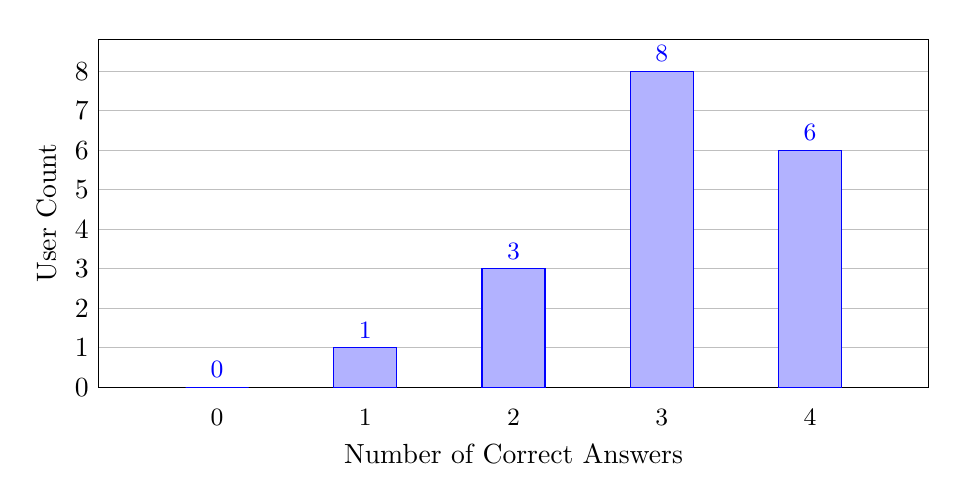
\begin{tikzpicture}
    \begin{axis}[
        ybar,
        width=\columnwidth,
        height=6cm,
        grid=both, % Set grid to both
        xmajorgrids=false, % Disable vertical grid lines
        ymajorgrids=true, % Enable horizontal grid lines
        ymin=0,
        xtick=data,
        xtick style={draw=none},
        ytick={0,1,2,3,4,5,6,7,8},
        ytick style={draw=none},
        xticklabel style={font=\small},
        xlabel={Number of Correct Answers},
        ylabel={User Count},
        bar width=0.8cm,
        enlarge x limits=0.2,
        nodes near coords,
        every node near coord/.append style={font=\small, rotate=0, anchor=south},
        ]
        \addplot coordinates {(0, 0) (1, 1) (2, 3) (3, 8) (4, 6)};
    \end{axis}
\end{tikzpicture}

\end{document}